%% tags: boldmath; network; graph; edgeLabels; externalImage
\PassOptionsToPackage{usenames,dvipsnames}{xcolor}
\documentclass[tikz,border=2]{standalone}
\usetikzlibrary{shadows,arrows,shapes,positioning,calc,backgrounds,fit}
%%
\definecolor{source}{HTML}{66C2A5}
\definecolor{sink}{HTML}{8DA0CB}
\definecolor{hub}{HTML}{FC8D62}
%%
% Define the layers to draw the diagram
\begin{document}
\begin{tikzpicture}
   [node distance=1cm,scale=2,
      vertex/.style={shape=circle,draw=black,inner sep=1pt,minimum
      size=.5cm,font=\boldmath},
lbl/.style={font=\small,inner sep=2pt},
trans/.style={ultra thick,black!40,text=black,midway},
gravity/.style={fill=white,font=\small,inner sep=2pt},
ledge/.style={thin,inner sep=2pt,>=latex, shorten >=1pt,
shorten <=1pt,looseness=.5},
gedge/.style={thin,inner sep=2pt,>=latex, shorten >=1pt,
shorten <=1pt,looseness=.5,red!60!black!60,text=black},
pedge/.style={trans,inner sep=2pt,>=latex, shorten >=1pt,
shorten <=1pt}]
%%
\newcommand{\xya}{(0,0)}
\newcommand{\xyb}{(1,-.5)}
\newcommand{\xyc}{(2,0)}
\newcommand{\xyd}{(0,-1.5)}
\newcommand{\xye}{(1.25,-2)}
\newcommand{\xyf}{(2.25,-1.75)}
%%
\begin{scope}
   \node [font=\Large] at (1.4,-3) {(a)}; %% Node attributes and
   %%    transportation network};
\node (a) [vertex,label=above:{$0,5$}] at \xya {$a$};
\node (b) [vertex,label=above:{$0,10$},fill=hub] at \xyb {$b$};
\node (c) [vertex,label=above:{$1,10$},fill=sink] at \xyc {$c$};
\node (d) [vertex,label=below:{$3,4$}] at \xyd {$d$};
\node (e) [vertex,label=below:{$4,2$}] at \xye {$e$};
\node (f) [vertex,label=below:{$15,2$},fill=source] at \xyf {$f$};
%%
\draw[trans] (a) -- (b) node [trans,above] {$1$};
\draw[trans] (b) -- (c) node [trans,above] {$1$};
\draw[trans] (b) -- (d) node [trans,left] {$3$};
\draw[trans] (b) -- (e) node (tt) [trans,right] {$4$};
\draw[trans] (d) -- (e) node [trans,above] {$2$};
\draw[trans] (e) -- (f) node [trans,above] {$1$};
%%
%% labels
\draw[ledge,<-] ($(c)+(.1,.35)$) -- +(.25,.25) node [lbl,label=above:Consumption] {};
\draw[ledge,<-] ($(c)+(-.2,.25)$) -- +(-.35,.15) node [lbl,label=above:Production] {};
\draw[ledge,<-] ($(tt)+(.1,0)$) -- +(.3,0) node [lbl,label=right:Travel time] {};
\draw[ledge,<-] ($(c)+(.1,-.1)$) -- +(.3,-.3) node [lbl,label=right:Sink] {};
\draw[ledge,<-] ($(b)+(-.15,0)$) -- +(-.3,0) node [lbl,label=left:Possible Hub] {};
\draw[ledge,<-] ($(f)+(.15,0)$) -- +(.35,0) node [lbl,label=right:Source] {};
\end{scope}
%%
\begin{scope}[shift={(4.5cm,0cm)}]
\node at (1.1,-.7) {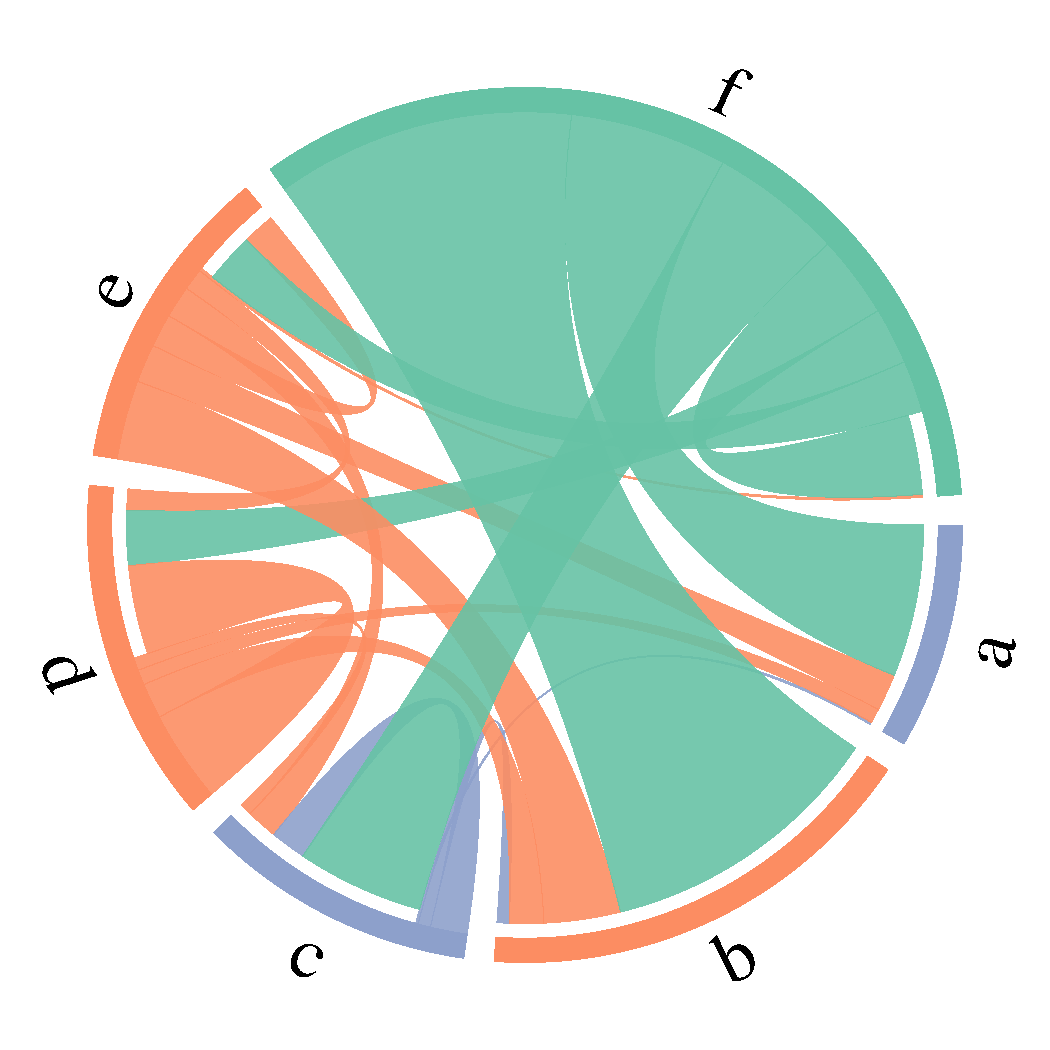
\includegraphics[width=7cm]{aux/example_flow.pdf}};
\node [] at (2.5,-2.3) {appears as sink};
\node [] at (-.7,.3) {appears as source};
\node [font=\Large] at (1.2,-3) {(b)}; %% Flow network};
\end{scope}
%%
\begin{scope}[shift={(9cm,0)}]
   \node [font=\Large] at (1.2,-3) {(c)};  %% Projected flow network};
\node (a) [vertex,label=above:{$h(a)=0$},fill=sink] at \xya {$a$};
\node (b) [vertex,label=below right:{$h(b)=0.87$},fill=hub] at \xyb {$b$};
\node (c) [vertex,label=above:{$h(c)=0$},fill=sink] at \xyc {$c$};
\node (d) [vertex,label=below left:{$h(d)=0.99$},fill=hub] at \xyd {$d$};
\node (e) [vertex,label=below:{$h(e)=0.999$},fill=hub] at \xye {$e$};
\node (f) [vertex,label=above:{$h(f)=0$},fill=source] at \xyf {$f$};
%%
\path[pedge] (b) edge[pedge,->] node [gravity] {$4.11$} (a);
\path[pedge] (b) edge[pedge,->] node [gravity] {$3.11$} (c);
\path[pedge] (d) edge[pedge,->] node [gravity] {$1.22$} (b);
\path[pedge] (e) edge[pedge,->] node [gravity] {$1.51$} (d);
\path[pedge] (e) edge[pedge,->] node [gravity] {$14.21$} (b);
\path[pedge] (f) edge[pedge,->] node [gravity] {$13.36$} (e);
\end{scope}
\end{tikzpicture}
\end{document}
